\documentclass[tikz]{standalone}
% Default preamble
\usepackage{pgfplots}
\pgfplotsset{compat=newest}
\usepgfplotslibrary{groupplots}
\usepgfplotslibrary{polar}
\usepgfplotslibrary{statistics}
\begin{document}
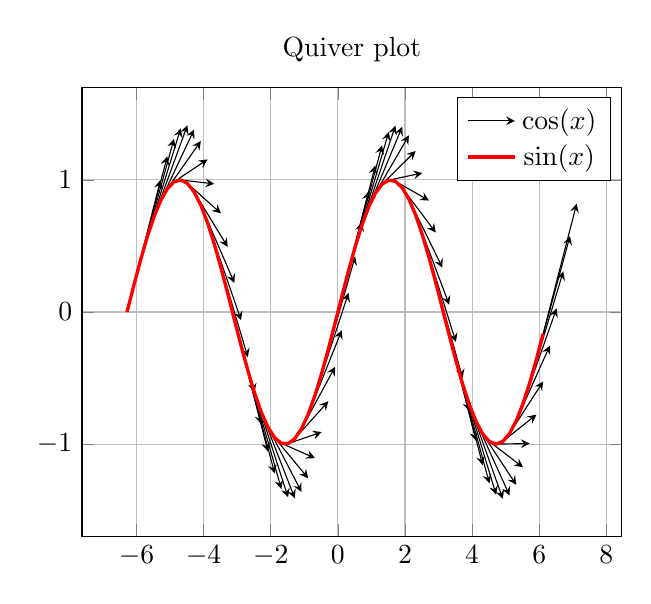
\begin{tikzpicture}[]
\begin{axis}[title={Quiver plot}, grid={both}]
    \addplot[quiver={u={\thisrow{u}}, v={\thisrow{v}}}, -stealth]
        table[row sep={\\}]
        {
            x  y  u  v  \\
            -6.283185307179586  2.4492935982947064e-16  1.0  1.0  \\
            -6.083185307179586  0.19866933079506163  1.0  0.9800665778412415  \\
            -5.883185307179586  0.389418342308651  1.0  0.9210609940028849  \\
            -5.683185307179587  0.5646424733950353  1.0  0.8253356149096783  \\
            -5.483185307179586  0.7173560908995228  1.0  0.6967067093471654  \\
            -5.283185307179586  0.8414709848078966  1.0  0.5403023058681395  \\
            -5.083185307179586  0.9320390859672265  1.0  0.3623577544766732  \\
            -4.883185307179586  0.9854497299884603  1.0  0.16996714290024034  \\
            -4.683185307179587  0.9995736030415052  1.0  -0.029199522301288618  \\
            -4.483185307179586  0.9738476308781951  1.0  -0.2272020946930871  \\
            -4.283185307179586  0.9092974268256816  1.0  -0.41614683654714263  \\
            -4.083185307179586  0.80849640381959  1.0  -0.588501117255346  \\
            -3.883185307179586  0.6754631805511505  1.0  -0.7373937155412459  \\
            -3.683185307179586  0.5155013718214639  1.0  -0.8568887533689474  \\
            -3.483185307179586  0.33498815015590444  1.0  -0.9422223406686583  \\
            -3.2831853071795862  0.141120008059867  1.0  -0.9899924966004455  \\
            -3.083185307179586  -0.05837414342758033  1.0  -0.998294775794753  \\
            -2.883185307179586  -0.2555411020268319  1.0  -0.9667981925794609  \\
            -2.683185307179586  -0.4425204432948527  1.0  -0.8967584163341469  \\
            -2.483185307179586  -0.6118578909427195  1.0  -0.7909677119144164  \\
            -2.2831853071795862  -0.7568024953079284  1.0  -0.6536436208636117  \\
            -2.083185307179586  -0.8715757724135883  1.0  -0.4902608213406992  \\
            -1.8831853071795859  -0.9516020738895161  1.0  -0.30733286997841913  \\
            -1.683185307179586  -0.9936910036334645  1.0  -0.11215252693505397  \\
            -1.483185307179586  -0.9961646088358407  1.0  0.08749898343944708  \\
            -1.283185307179586  -0.9589242746631383  1.0  0.2836621854632267  \\
            -1.083185307179586  -0.883454655720153  1.0  0.46851667130037733  \\
            -0.8831853071795859  -0.772764487555987  1.0  0.6346928759426348  \\
            -0.6831853071795859  -0.6312666378723208  1.0  0.7755658785102502  \\
            -0.4831853071795859  -0.4646021794137567  1.0  0.8855195169413193  \\
            -0.2831853071795859  -0.2794154981989253  1.0  0.9601702866503662  \\
            -0.08318530717958589  -0.083089402817496  1.0  0.9965420970232175  \\
            0.11681469282041412  0.11654920485049389  1.0  0.9931849187581926  \\
            0.31681469282041413  0.31154136351337874  1.0  0.9502325919585293  \\
            0.5168146928204141  0.4941133511386089  1.0  0.8693974903498248  \\
            0.7168146928204142  0.6569865987187896  1.0  0.7539022543433042  \\
            0.9168146928204142  0.7936678638491534  1.0  0.6083513145322541  \\
            1.1168146928204141  0.898708095811627  1.0  0.43854732757439013  \\
            1.3168146928204143  0.9679196720314867  1.0  0.25125984258225464  \\
            1.5168146928204143  0.998543345374605  1.0  0.05395542056264884  \\
            1.7168146928204142  0.9893582466233817  1.0  -0.1455000338086142  \\
            1.9168146928204142  0.9407305566797727  1.0  -0.3391548609838358  \\
            2.116814692820414  0.8545989080882803  1.0  -0.5192886541166858  \\
            2.3168146928204143  0.7343970978741126  1.0  -0.6787200473200132  \\
            2.5168146928204145  0.5849171928917615  1.0  -0.8110930140616561  \\
            2.716814692820414  0.4121184852417559  1.0  -0.9111302618846773  \\
            2.9168146928204144  0.2228899141002461  1.0  -0.9748436214041639  \\
            3.116814692820414  0.024775425453357522  1.0  -0.9996930420352065  \\
            3.3168146928204143  -0.17432678122298076  1.0  -0.9846878557941268  \\
            3.5168146928204145  -0.36647912925192866  1.0  -0.9304262721047531  \\
            3.716814692820414  -0.5440211108893704  1.0  -0.8390715290764521  \\
            3.9168146928204144  -0.6998746875935435  1.0  -0.7142656520271992  \\
            4.116814692820414  -0.8278264690856538  1.0  -0.5609842574272286  \\
            4.316814692820414  -0.922775421612807  1.0  -0.3853381907718286  \\
            4.5168146928204145  -0.9809362300664916  1.0  -0.19432990645533454  \\
            4.716814692820415  -0.9999902065507035  1.0  0.004425697988051919  \\
            4.916814692820415  -0.979177729151317  1.0  0.20300486381875238  \\
            5.116814692820414  -0.9193285256646756  1.0  0.3934908663478911  \\
            5.316814692820414  -0.8228285949687082  1.0  0.5682896297679746  \\
            5.5168146928204145  -0.6935250847771222  1.0  0.7204324789908388  \\
            5.716814692820415  -0.536572918000434  1.0  0.8438539587324927  \\
            5.916814692820415  -0.3582292822368268  1.0  0.933633644074638  \\
            6.116814692820414  -0.16560417544830916  1.0  0.9861923022788637  \\
        }
        ;
    \addlegendentry[] {$\cos(x)$}
    \addplot[color={red}, very thick]
        coordinates {
            (-6.283185307179586, 2.4492935982947064e-16)
            (-6.083185307179586, 0.19866933079506163)
            (-5.883185307179586, 0.389418342308651)
            (-5.683185307179587, 0.5646424733950353)
            (-5.483185307179586, 0.7173560908995228)
            (-5.283185307179586, 0.8414709848078966)
            (-5.083185307179586, 0.9320390859672265)
            (-4.883185307179586, 0.9854497299884603)
            (-4.683185307179587, 0.9995736030415052)
            (-4.483185307179586, 0.9738476308781951)
            (-4.283185307179586, 0.9092974268256816)
            (-4.083185307179586, 0.80849640381959)
            (-3.883185307179586, 0.6754631805511505)
            (-3.683185307179586, 0.5155013718214639)
            (-3.483185307179586, 0.33498815015590444)
            (-3.2831853071795862, 0.141120008059867)
            (-3.083185307179586, -0.05837414342758033)
            (-2.883185307179586, -0.2555411020268319)
            (-2.683185307179586, -0.4425204432948527)
            (-2.483185307179586, -0.6118578909427195)
            (-2.2831853071795862, -0.7568024953079284)
            (-2.083185307179586, -0.8715757724135883)
            (-1.8831853071795859, -0.9516020738895161)
            (-1.683185307179586, -0.9936910036334645)
            (-1.483185307179586, -0.9961646088358407)
            (-1.283185307179586, -0.9589242746631383)
            (-1.083185307179586, -0.883454655720153)
            (-0.8831853071795859, -0.772764487555987)
            (-0.6831853071795859, -0.6312666378723208)
            (-0.4831853071795859, -0.4646021794137567)
            (-0.2831853071795859, -0.2794154981989253)
            (-0.08318530717958589, -0.083089402817496)
            (0.11681469282041412, 0.11654920485049389)
            (0.31681469282041413, 0.31154136351337874)
            (0.5168146928204141, 0.4941133511386089)
            (0.7168146928204142, 0.6569865987187896)
            (0.9168146928204142, 0.7936678638491534)
            (1.1168146928204141, 0.898708095811627)
            (1.3168146928204143, 0.9679196720314867)
            (1.5168146928204143, 0.998543345374605)
            (1.7168146928204142, 0.9893582466233817)
            (1.9168146928204142, 0.9407305566797727)
            (2.116814692820414, 0.8545989080882803)
            (2.3168146928204143, 0.7343970978741126)
            (2.5168146928204145, 0.5849171928917615)
            (2.716814692820414, 0.4121184852417559)
            (2.9168146928204144, 0.2228899141002461)
            (3.116814692820414, 0.024775425453357522)
            (3.3168146928204143, -0.17432678122298076)
            (3.5168146928204145, -0.36647912925192866)
            (3.716814692820414, -0.5440211108893704)
            (3.9168146928204144, -0.6998746875935435)
            (4.116814692820414, -0.8278264690856538)
            (4.316814692820414, -0.922775421612807)
            (4.5168146928204145, -0.9809362300664916)
            (4.716814692820415, -0.9999902065507035)
            (4.916814692820415, -0.979177729151317)
            (5.116814692820414, -0.9193285256646756)
            (5.316814692820414, -0.8228285949687082)
            (5.5168146928204145, -0.6935250847771222)
            (5.716814692820415, -0.536572918000434)
            (5.916814692820415, -0.3582292822368268)
            (6.116814692820414, -0.16560417544830916)
        }
        ;
    \addlegendentry[] {$\sin(x)$}
\end{axis}
\end{tikzpicture}
\end{document}
